% !TEX root = cap02_standalone.tex
% Capítulo 2. Marco teórico
% Estructura según índice de la Dra. Lárraga.
\graphicspath{{figures/}{../figures/}}

\chapter{Marco teórico}
\label{ch:marco-teorico}

\begin{resumen}
Este marco teórico sigue el orden del flujo descrito en el Cap.~\ref{ch:introduccion}: primero los algoritmos de preprocesamiento de imágenes (StandardScaler, PCA, K-Means y SVM), después la definición formal del autómata celular probabilístico y el método de Pesos de Evidencia como función de transición, y al final las métricas espaciales de evaluación. Cada sección incluye únicamente los conceptos que el modelo del Cap.~\ref{ch:modelo-crecimiento-urbano} efectivamente utiliza.
\end{resumen}


% ============================================================
\section{Fundamentos del preprocesamiento de imágenes}
\label{sec:preprocesamiento-datos}
% ============================================================

% TODO-REDACCION: esta sección debe contener SOLO conceptos, cada uno en su propia subsección, con
% cita del .bib ya verificado e indicando si el método es supervisado o no supervisado. El material
% metodológico de este trabajo (adquisición, arreglo M_{t,i,j}, las 23 características por píxel, el
% pipeline aplicado y su figura) se trasladó a la Sección~\ref{sec:preprocesamiento} del
% Capítulo~\ref{ch:modelo-crecimiento-urbano}.
% Quedan por redactar aquí, como subsecciones conceptuales previas a los algoritmos:
%   - imágenes satelitales y Google Earth como fuente de datos geoespaciales;
%   - clasificación de cobertura del suelo y el caso binario urbano/no-urbano;
%   - espacio de color RGB y transformaciones cromáticas (CIE L*a*b*, HSV);
%   - patrones binarios locales (LBP) como descriptor de textura.
% Cada subsección debe cerrar con una liga al capítulo donde se aplica.


	
	
\subsection{Estandarización y análisis de componentes principales}

La reducción dimensional se apoya en una proyección lineal de las variables estandarizadas sobre un subespacio de menor dimensión:

\begin{equation}
\mathbf{f}(x,y) = \mathbf{W} \mathbf{f}(x,y)
\label{eq:pca_formula}
\end{equation}

donde $\mathbf{W}$ es la matriz de pesos PCA.

A continuación se define el algoritmo de StandardScaler y PCA.

\begin{algorithm}[H]
	\caption{StandardScaler: estandarización por z-score}
	\label{alg:standard-scaler}
	\begin{algorithmic}[1]
	\Require Matriz de features $X \in \mathbb{R}^{N \times F}$ ($N$ píxeles, $F$ features)
	\Ensure  Matriz estandarizada $\tilde{X} \in \mathbb{R}^{N \times F}$
	
	\State \textbf{Fase de ajuste} (sobre los datos de entrenamiento)
	\For{$j = 1$ \textbf{to} $F$}
		\State $\mu_j \leftarrow \dfrac{1}{N}\sum_{i=1}^{N} X_{ij}$
		\State $\sigma_j \leftarrow \sqrt{\dfrac{1}{N}\sum_{i=1}^{N}(X_{ij} - \mu_j)^2}$
	\EndFor
	
	\State \textbf{Fase de transformación}
	\For{$i = 1$ \textbf{to} $N$}
		\For{$j = 1$ \textbf{to} $F$}
			\State $\tilde{X}_{ij} \leftarrow \dfrac{X_{ij} - \mu_j}{\sigma_j + \varepsilon}$
			\Comment{$\varepsilon$ evita división por cero}
		\EndFor
	\EndFor
	\State \Return $\tilde{X}$
	\end{algorithmic}
	\end{algorithm}
	
	\begin{algorithm}[H]
	\caption{PCA: reducción de dimensionalidad}
	\label{alg:pca}
	\begin{algorithmic}[1]
	\Require Matriz estandarizada $\tilde{X} \in \mathbb{R}^{N \times F}$,
			 número de componentes $k=8$
	\Ensure  Representación reducida $Z \in \mathbb{R}^{N \times k}$
	
	\State Calcular la matriz de covarianza:
		   $\Sigma \leftarrow \dfrac{1}{N-1}\,\tilde{X}^\top \tilde{X}$
	\State Obtener descomposición espectral:
		   $\Sigma\,\mathbf{w}_j = \lambda_j\,\mathbf{w}_j$,
		   \quad $j = 1,\ldots,F$
	\State Ordenar autovalores de forma descendente:
		   $\lambda_1 \ge \lambda_2 \ge \cdots \ge \lambda_F$
	\State Seleccionar los $k$ autovectores de mayor varianza:
		   $\mathbf{W} = [\mathbf{w}_1\;\mathbf{w}_2\;\cdots\;\mathbf{w}_k]
		   \in \mathbb{R}^{F \times k}$
	\State Proyectar los datos:
		   $Z \leftarrow \tilde{X}\,\mathbf{W}$
	\State \Return $Z$
	\end{algorithmic}
\end{algorithm}

\subsection{Agrupamiento K-Means}

% TODO-REDACCION: añadir la cita del método y explicitar que es no supervisado.
El agrupamiento K-Means particiona un conjunto de observaciones en $k$ grupos minimizando la suma de distancias cuadradas de cada punto al centroide de su grupo. Su definición es la siguiente:

\begin{algorithm}[H]
	\caption{K-Means: agrupamiento no supervisado ($k=2$)}
	\label{alg:kmeans}
	\begin{algorithmic}[1]
	\Require Matriz PCA $Z \in \mathbb{R}^{N \times 8}$, número de clústeres $k=2$,
			 inicializaciones $n_{\text{init}}=10$
	\Ensure  Vector de etiquetas $\ell \in \{0,1\}^N$
	\For{cada inicialización $r = 1,\ldots,n_{\text{init}}$}
		\State Inicializar centroides $\{\mu_1, \mu_2\} \subset Z$ (selección aleatoria)
		\Repeat
			\State \textbf{Asignación:} $\ell_i \leftarrow \arg\min_{c \in \{1,2\}}
				   \|z_i - \mu_c\|_2^2 \quad \forall\, i$
			\State \textbf{Actualización:}
				   $\mu_c \leftarrow \dfrac{1}{|\mathcal{C}_c|}\sum_{i \in \mathcal{C}_c} z_i
				   \quad \forall\, c$,
				   donde $\mathcal{C}_c = \{i : \ell_i = c\}$
		\Until{los centroides no cambien}
		\State Registrar inercia $\mathcal{J}_r = \sum_{i=1}^N \|z_i - \mu_{\ell_i}\|_2^2$
	\EndFor
	\State Seleccionar la solución con menor $\mathcal{J}_r$
	\State \Return $\ell$
	\end{algorithmic}
\end{algorithm}
	
\subsection{Máquinas de vectores de soporte}

% TODO-REDACCION: añadir la cita del método y explicitar que es supervisado, señalando que aquí se
% entrena sobre pseudo-etiquetas y no sobre verdad terreno.
Las pseudo-etiquetas producidas por un agrupamiento no supervisado pueden emplearse como verdad base
para entrenar un clasificador de máquina de vectores de soporte, que después predice la etiqueta del
resto de las observaciones.

\begin{algorithm}[H]
\caption{SVM lineal: clasificación sobre pseudo-etiquetas K-Means}
\label{alg:svm}
\begin{algorithmic}[1]
\Require Matriz PCA $Z \in \mathbb{R}^{N \times 8}$,
         pseudo-etiquetas $\ell \in \{0,1\}^N$,
         tamaño de muestra $n_s = \min(N,\,10\,000)$
\Ensure  Mapa de clasificación $\hat{y} \in \{0,1\}^{H \times W}$
\State Seleccionar submuestra aleatoria $\mathcal{S} \subset \{1,\ldots,N\}$,
       $|\mathcal{S}| = n_s$
\State Entrenar SVM lineal minimizando:
\[
\min_{\mathbf{w},\,b}\; \frac{1}{2}\|\mathbf{w}\|^2 + C\sum_{i \in \mathcal{S}}
\max\!\left(0,\;1 - \ell_i^*\bigl(\mathbf{w}^\top z_i + b\bigr)\right)
\]
donde $\ell_i^* \in \{-1,+1\}$ es la pseudo-etiqueta recodificada
\State \textbf{Predicción sobre todos los píxeles:}
       $\hat{y}_i \leftarrow \text{sign}\!\left(\mathbf{w}^\top z_i + b\right)
       \quad \forall\, i \in \{1,\ldots,N\}$
\State Recodificar a binario: $\hat{y}_i \leftarrow \mathbf{1}[\hat{y}_i > 0]$
\State Reorganizar en mapa $H \times W$
\State \Return $\hat{y}$
\end{algorithmic}
\end{algorithm}


% ============================================================
\section{Autómatas Celulares}
\label{sec:automatas-celulares}
% ============================================================

Un \textbf{Autómata Celular} (AC), en el sentido formalizado por \textcite{Wolfram1984}, es un sistema dinámico discreto definido sobre una cuadrícula regular de $N$ celdas. Formalmente, un AC queda definido por la cuádrupla $(Q, \mathcal{N}, \delta, q_0)$. El primer elemento, $Q$, es el conjunto finito de estados posibles de cada celda; en este trabajo $Q = \{0, 1\}$ distingue lo no-urbano de lo urbano. El segundo, $\mathcal{N}$, es la vecindad: el conjunto de celdas adyacentes cuyo estado influye en la transición. El tercero, $\delta: Q^{|\mathcal{N}|} \to Q$, es la función de transición, que determina el nuevo estado de una celda a partir del estado de sus vecinos. El último, $q_0: \Omega \to Q$, fija la configuración inicial del sistema.

En el contexto del crecimiento urbano, el dominio espacial $\Omega \subset \mathbb{Z}^2$ es una cuadrícula discreta de celdas indexadas por pares $(i,j)$, donde $i \in \{1,\ldots,R\}$ indica la fila y $j \in \{1,\ldots,C\}$ la columna, con $N = R \times C$ celdas en total.

En los AC probabilísticos, la función de transición $\delta$ asigna probabilidades a cada posible nuevo estado, en lugar de determinar el siguiente estado de forma determinista. Esta extensión, base de los modelos urbanos basados en AC desde \textcite{White1997} y de marcos calibrados como SLEUTH \parencite{Clarke1998}, resulta adecuada para el modelado urbano, en el que la transición de no-urbano a urbano no está garantizada incluso cuando las condiciones locales son favorables.

% TODO-REDACCION: definición de SLEUTH traída del Capítulo~\ref{ch:estado-del-arte} por indicación de
% la Dra. Lárraga (el concepto va en el marco teórico; el análisis de lo hecho con SLEUTH se queda en
% el estado del arte). Verificar y citar la expansión del acrónimo.
Entre los marcos de autómatas celulares urbanos, SLEUTH \parencite{Clarke1998} es el más difundido. Su nombre resume las capas de entrada que utiliza (\textit{slope}, \textit{land use}, \textit{exclusion}, \textit{urban}, \textit{transportation} y \textit{hillshade}) y su comportamiento queda gobernado por cinco coeficientes de crecimiento (\emph{diffusion}, \emph{breed}, \emph{spread}, \emph{slope resistance} y \emph{road gravity}) que se ajustan mediante búsqueda sobre un espacio discreto de combinaciones, evaluando cada una con simulaciones Monte Carlo. Las dificultades prácticas de esa calibración se discuten en el Capítulo~\ref{ch:estado-del-arte}.

Los dos tipos de vecindad más utilizados en modelado urbano son la vecindad de Von Neumann (cuatro celdas ortogonales) y la vecindad de Moore (ocho celdas incluyendo diagonales). En ambos casos, el radio de influencia puede extenderse más allá de la celda inmediatamente adyacente, permitiendo capturar efectos de accesibilidad y proximidad a zonas urbanas existentes.

Para el presente modelo, la influencia de la vecindad se cuantifica mediante la proporción de celdas urbanas en un radio $r$ alrededor de la celda evaluada:

\begin{equation}
\Omega_{i,j}(r) = \frac{1}{|\mathcal{N}_{i,j}(r)|} \sum_{(i',j') \in \mathcal{N}_{i,j}(r)} s_{i',j'}
\label{eq:neighborhood}
\end{equation}

donde $s_{i',j'} \in \{0,1\}$ es el estado urbano de la celda vecina en posición $(i',j')$ y $\mathcal{N}_{i,j}(r)$ es el conjunto de celdas dentro del radio $r$ alrededor de la celda $(i,j)$. Dicho de otra forma, es la proporción de celdas urbanas en el radio $r$ alrededor de la celda $(i,j)$, bajo la definición de vecindad.

La probabilidad de que una celda no-urbana en posición $(i,j)$ transite al estado urbano en el paso $t+1$ se define como una función de tres componentes:

\begin{equation}
P(s_{i,j}^{t+1} = 1 \mid s_{i,j}^t = 0) = f\!\left(W_{i,j},\; \Omega_{i,j}(r),\; \varepsilon_{i,j}\right)
\label{eq:transition_prob}
\end{equation}

donde $W_{i,j}$ es la idoneidad espacial asignada por el método WoE (definida a continuación), $\Omega_{i,j}(r)$ es el efecto de vecindad, y $\varepsilon_{i,j}$ es un término estocástico que introduce variabilidad aleatoria en la simulación. La función $f$ combina estos tres factores según parámetros que, en este trabajo, se ajustan mediante el procedimiento de calibración descrito en el Capítulo~\ref{ch:modelo-crecimiento-urbano} y en la Sección~\ref{sec:calibracion-narrativa}. Esta función es la que define la transición de una celda no-urbana a una urbana.

% ============================================================
\section{Pesos de Evidencia}
\label{sec:woe}
% ============================================================

% TODO-REDACCION: la definición conceptual de WoE ya vivía dentro de la sección de autómatas
% celulares y aquí se promueve a sección propia, como pidió la Dra. Lárraga. Falta añadir sus
% ventajas y limitaciones, la justificación de por qué se combina WoE con un autómata celular para
% calibrar la regla de transición, y la interpretación explícita de la Figura~\ref{fig:concepto-woe}.
El método de \textbf{Pesos de Evidencia} (Weight of Evidence, WoE) es una técnica estadística de origen bayesiano que cuantifica la asociación entre una variable espacial y la ocurrencia de un evento, en este caso la transición de suelo no-urbano a urbano \parencite{BonhamCarter1994}. Fue desarrollado originalmente en el contexto de la predicción de depósitos minerales y posteriormente adaptado al análisis de cambio de uso de suelo. 

Para una variable espacial $X$ discretizada en categorías o intervalos, el peso de evidencia de la categoría $b$ se define como:

\begin{equation}
W^+(b) = \ln \frac{P(X = b \mid \text{transición})}{P(X = b \mid \text{no transición})}
\label{eq:woe}
\end{equation}

donde $P(X \in b \mid \text{transición})$ es la proporción de píxeles con transición observada que pertenecen a la categoría $b$, y $P(X \in b \mid \text{no transición})$ es la proporción equivalente para píxeles sin transición. Los pesos positivos indican que la categoría $b$ favorece la transición; los pesos negativos indican lo contrario. En esta expresión, $b$ no representa la clase urbano/no-urbano, sino una categoría, intervalo o bin de la variable espacial $X$ (por ejemplo, un rango de distancia a la mancha urbana existente o un rango de densidad vecinal). La clase binaria $\{0,1\}$ corresponde al estado observado o predicho de la celda, mientras que las categorías $b$ pertenecen al espacio de valores de cada variable explicativa.

El peso total para la celda en posición $(i,j)$ se obtiene sumando los pesos de cada variable espacial evaluada en esa celda:

\begin{equation}
W_{i,j} = \sum_{k=1}^{V} W^+(b_{(i,j)k})
\label{eq:woe_total}
\end{equation}

donde $V$ es el número de variables espaciales consideradas y $b_{(i,j)k}$ es la categoría o intervalo que toma la variable espacial $k$ en la celda $(i,j)$. En la implementación de este trabajo, $V = 7$, porque se consideran siete variables espaciales derivadas de la configuración urbana histórica. Por tanto, $V$ no es el número de clases del mapa binario; las clases del estado celular siguen siendo dos ($0$ para no urbano y $1$ para urbano). Este valor $W_{i,j}$ se transforma mediante una función sigmoide para obtener una probabilidad de transición acotada en $[0,1]$:

\begin{equation}
P_{i,j}^{\text{WoE}} = \frac{1}{1 + e^{-W_{i,j}}}
\label{eq:woe_sigmoid}
\end{equation}

\begin{figure}[htbp]
  \centering
  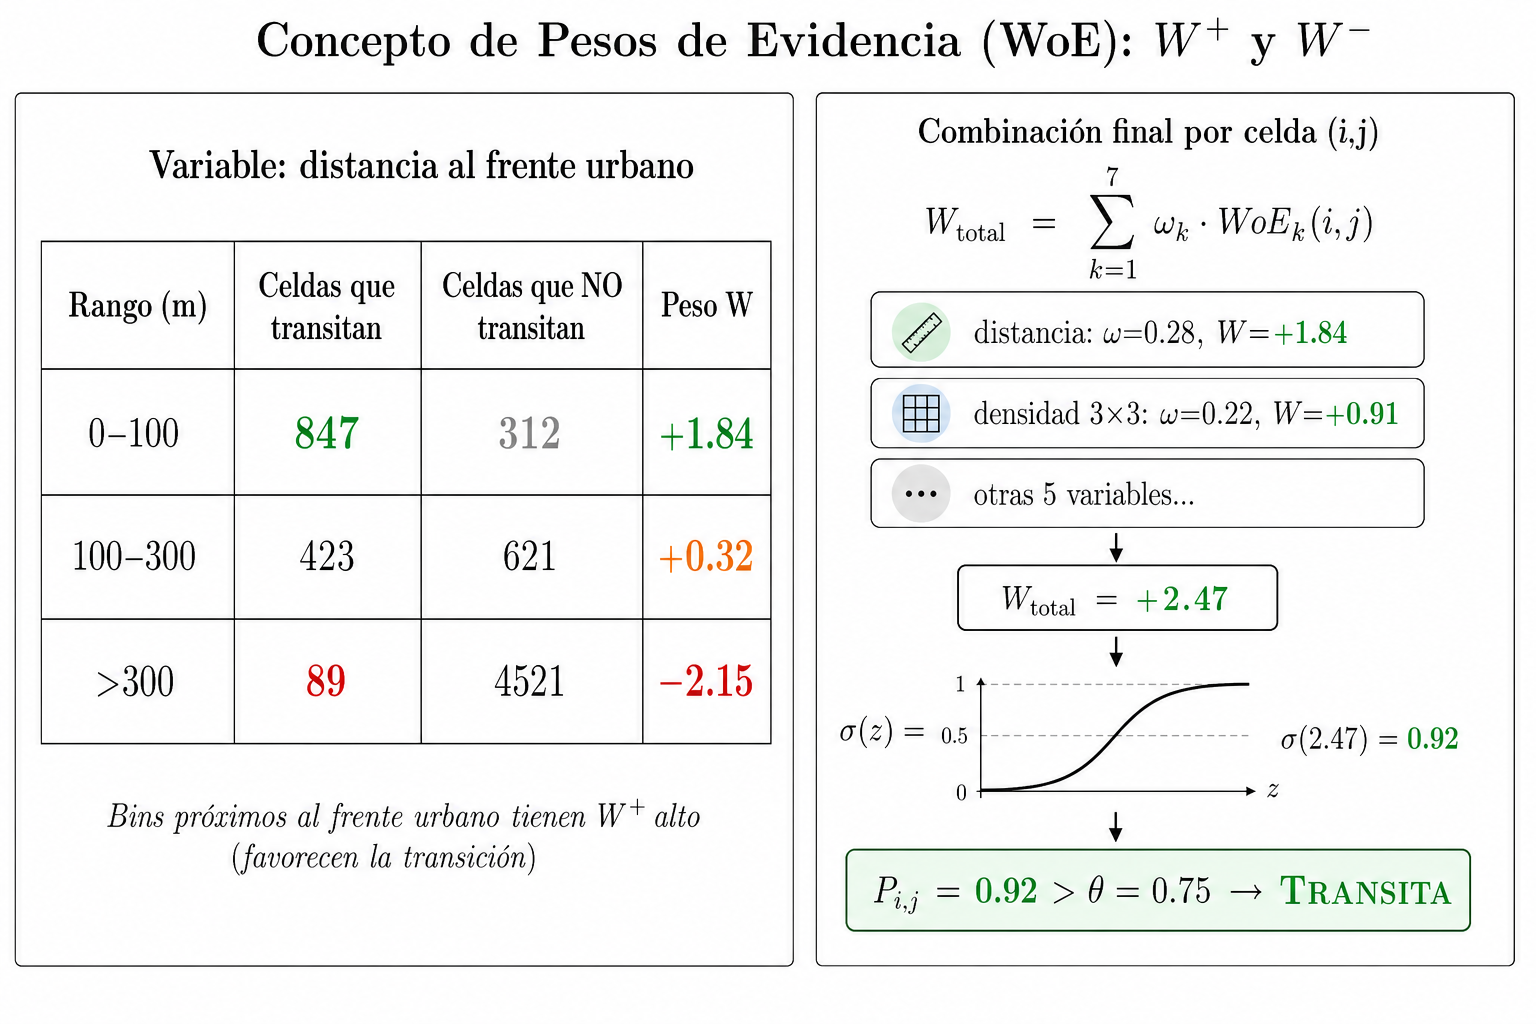
\includegraphics[width=0.95\linewidth]{F9_concepto_woe_ai}
  \caption{Ejemplo del cálculo de WoE: la variable \textit{distancia al frente urbano} acumula pesos positivos en bins próximos y negativos en bins lejanos. La suma ponderada pasa por la sigmoide y se compara con $\theta=0{,}75$.}
  \label{fig:concepto-woe}
\end{figure}

Una propiedad relevante del WoE es su interpretabilidad: cada peso $W^+(b)$ puede traducirse en términos geográficos. Por ejemplo, si la variable \textit{distancia a manchas urbanas} tiene un peso negativo para distancias grandes, ello sugiere menor probabilidad de urbanización en celdas alejadas de vías de comunicación. Dicha transparencia puede apoyar la comunicación de resultados a planificadores urbanos, sin sustituir el juicio experto ni las políticas públicas aplicables en cada contexto.

El cálculo de los pesos se realiza sobre datos históricos de transición, lo que hace que las probabilidades resultantes reflejen empíricamente los patrones observados en el área de estudio, en lugar de depender de supuestos teóricos sobre el comportamiento urbano.

% ============================================================
\section{Métricas de evaluación de modelos predictivos}
% ============================================================

La evaluación cuantitativa del desempeño del modelo requiere métricas que comparen el mapa predicho con el mapa observado a nivel de píxel y a nivel global. A continuación se presentan las métricas utilizadas en este trabajo, derivadas de la matriz de confusión espacial. La matriz de confusión es una tabla que muestra el número de píxeles correctamente clasificados y los errores de clasificación.

Sea $\Omega \subset \mathbb{R}^2$ el dominio espacial de estudio discretizado en $N = |\Omega|$ píxeles. Para cada píxel $i \in \Omega$, sea $y_i \in \{0, 1\}$ el estado observado real (donde 0 denota no-urbano y 1 denota urbano), y sea $\hat{y}_i \in \{0, 1\}$ el estado predicho por el modelo. En esta notación, $i$ es un índice lineal sobre las $N = R \times C$ celdas de la cuadrícula; cada valor $i$ corresponde a la celda en posición $(r,c)$ con $r \in \{1,\ldots,R\}$ filas y $c \in \{1,\ldots,C\}$ columnas. Se emplea el índice lineal por claridad en la notación de conjuntos; la equivalencia con la indexación bidimensional $(i,j)$ de las secciones anteriores es $i \leftrightarrow (r,c)$.

La \textbf{matriz de confusión} $\mathbf{C} \in \mathbb{N}^{2 \times 2}$ cuantifica la concordancia píxel a píxel entre predicción y observación:

\begin{equation}
\mathbf{C} = \begin{pmatrix}
TN & FP \\
FN & TP
\end{pmatrix}
\label{eq:confusion_matrix}
\end{equation}

donde los elementos se definen mediante la función indicadora $\mathbb{1}[\cdot]$ como sigue:

\begin{align}
TP &= \sum_{i \in \Omega} \mathbb{1}[\hat{y}_i = 1 \land y_i = 1] \quad \text{(verdaderos positivos: urbano predicho y observado)} \\
TN &= \sum_{i \in \Omega} \mathbb{1}[\hat{y}_i = 0 \land y_i = 0] \quad \text{(verdaderos negativos: no-urbano predicho y observado)} \\
FP &= \sum_{i \in \Omega} \mathbb{1}[\hat{y}_i = 1 \land y_i = 0] \quad \text{(falsos positivos: sobre-predicción)} \\
FN &= \sum_{i \in \Omega} \mathbb{1}[\hat{y}_i = 0 \land y_i = 1] \quad \text{(falsos negativos: sub-predicción)}
\end{align}

Estos cuatro componentes satisfacen $TP + TN + FP + FN = N$. La magnitud relativa de $FP$ frente a $FN$ revela el sesgo sistemático del modelo: si $FP > FN$, el modelo sobre-predice urbanización; si $FN > FP$, el modelo es conservador.

La construcción de la matriz requiere correspondencia espacial exacta entre los mapas predicho y observado: idéntica resolución espacial, sistema de proyección cartográfica y extensión geográfica. Los píxeles se clasifican evaluando las condiciones lógicas anteriores sobre todos los píxeles del dominio. La \textbf{exactitud global} mide la fracción de píxeles correctamente clasificados:

\begin{equation}
\text{Accuracy} = \frac{TP + TN}{N}
\label{eq:accuracy}
\end{equation}

Esta métrica es sensible al desbalance de clases. En contextos urbanos, donde la mayoría de píxeles no experimenta cambio, un modelo que predice ``no cambio'' en todos los píxeles obtiene Accuracy muy alta sin capturar ninguna dinámica. Por esta razón, Accuracy debe complementarse con métricas específicas para las transiciones. La \textbf{precisión} cuantifica la confiabilidad de las predicciones positivas:

\begin{equation}
\text{Precision} = \frac{TP}{TP + FP}
\label{eq:precision}
\end{equation}

Probabilísticamente, Precision estima $P(y_i = 1 \mid \hat{y}_i = 1)$: dado que el modelo predijo urbanización, ¿cuál es la probabilidad de que realmente ocurrió? Precision decrece cuando el modelo genera muchas falsas alarmas (sobre-predicción). Es especialmente relevante cuando el sobre-dimensionamiento de infraestructura tiene costos significativos. El \textbf{recall} cuantifica la capacidad de detectar píxeles con transición real:

\begin{equation}
\text{Recall} = \frac{TP}{TP + FN}
\label{eq:recall}
\end{equation}

Recall estima $P(\hat{y}_i = 1 \mid y_i = 1)$: dado que un píxel se urbanizó, ¿cuál es la probabilidad de que el modelo lo detectó? Recall bajo indica que el modelo omite transiciones reales, subestimando la expansión urbana.

Existe una tensión inherente entre Precision y Recall: aumentar el umbral de decisión tiende a incrementar Precision pero disminuye Recall, y viceversa. Esta dualidad motiva la siguiente métrica. El \textbf{F1-Score} es la media armónica entre Precision y Recall:

\begin{equation}
F1 = 2 \cdot \frac{\text{Precision} \cdot \text{Recall}}{\text{Precision} + \text{Recall}} = \frac{2 \cdot TP}{2 \cdot TP + FP + FN}
\label{eq:f1}
\end{equation}

La media armónica penaliza más severamente los valores bajos que la media aritmética, de modo que F1 es bajo cuando cualquiera de las dos métricas es baja, exigiendo buen desempeño en ambas dimensiones simultáneamente. El \textbf{coeficiente Kappa de Cohen}~\parencite{Cohen1960} corrige la concordancia observada por la concordancia esperada por azar:

\begin{equation}
\kappa = \frac{p_o - p_e}{1 - p_e}
\label{eq:kappa}
\end{equation}

donde $p_o = \text{Accuracy}$ es la proporción observada de concordancia, y $p_e$ es la proporción esperada por azar:

\begin{equation}
p_e = \frac{(TP + FP)(TP + FN) + (TN + FN)(TN + FP)}{N^2}
\label{eq:pe}
\end{equation}

El rango es $\kappa \in [-1, 1]$. Conforme a la escala de interpretación de uso común propuesta por \textcite{LandisKoch1977}, $\kappa > 0{,}81$ indica acuerdo casi perfecto; $0{,}61$--$0{,}80$, acuerdo sustancial; $0{,}41$--$0{,}60$, acuerdo moderado; $0{,}21$--$0{,}40$, acuerdo justo; y $\kappa < 0{,}20$, acuerdo pobre. La ventaja del coeficiente $\kappa$ frente a la \textit{Accuracy} es que proporciona una evaluación más realista ante desbalance de clases, al descontar el acuerdo esperado por azar.

Las métricas anteriores evalúan la concordancia global píxel a píxel, incluyendo tanto las transiciones como las permanencias. Sin embargo, en modelación de cambio de uso de suelo interesa específicamente predecir las \textbf{transiciones}, no las permanencias. Dado que la clase mayoritaria (píxeles sin cambio) puede inflar artificialmente las métricas globales, el \textbf{Figure of Merit} (FoM), propuesto como métrica comparable entre estudios de cambio de uso de suelo por \textcite{pontius2008comparing}, aborda esta limitación evaluando exclusivamente la predicción de cambio.

En un sistema urbano consolidado con $95\%$ de territorio permanente y $5\%$ con transición, un modelo trivial que predice ``no cambio'' obtiene \textit{Accuracy} $= 0{,}95$ sin capturar ninguna dinámica urbana. El FoM evalúa únicamente el subconjunto de píxeles donde ocurren transiciones, ignorando la clase mayoritaria.

Sea $\mathcal{T}_{obs}$ el conjunto de píxeles con cambio observado y $\mathcal{T}_{pred}$ el conjunto con cambio predicho entre $t_0$ y $t_1$. El FoM es el índice de Jaccard aplicado exclusivamente a las transiciones:

\begin{equation}
\text{FoM} = \frac{|\mathcal{T}_{obs} \cap \mathcal{T}_{pred}|}{|\mathcal{T}_{obs} \cup \mathcal{T}_{pred}|}
\label{eq:fom_jaccard}
\end{equation}

Descomponiendo en componentes:

\begin{align}
B &= |\mathcal{T}_{obs} \cap \mathcal{T}_{pred}| \quad \text{(cambio correctamente predicho)} \\
C &= |\mathcal{T}_{obs} \setminus \mathcal{T}_{pred}| \quad \text{(cambio observado no predicho: omisión)} \\
A &= |\mathcal{T}_{pred} \setminus \mathcal{T}_{obs}| \quad \text{(cambio predicho no observado: comisión)}
\end{align}

\begin{equation}
\boxed{\text{FoM} = \frac{B}{A + B + C}}
\label{eq:fom_formula}
\end{equation}

El denominador contiene exactamente tres términos. No incluye el término $D$ (píxeles sin cambio) porque FoM evalúa exclusivamente las transiciones.

% TODO-REDACCION: subseccionar esta sección como pidió la Dra. Lárraga (matriz de confusión;
% métricas de clasificación: exactitud, precisión, sensibilidad y F1; métricas de cambio: FoM, IoU y
% descomposición de Pontius), abriendo cada bloque con qué mide, para qué sirve y qué limitaciones
% tiene. Los dos párrafos siguientes se trasladaron desde el Capítulo~\ref{ch:estado-del-arte},
% donde eran definiciones conceptuales dentro de la discusión de la literatura.
La \textbf{Intersection over Union} (IoU) sobre la clase urbana provee información complementaria al FoM: mientras el FoM evalúa la calidad de la predicción del cambio, la IoU evalúa la calidad de la predicción del estado urbano final. Reportar ambas evita el sesgo de evaluar solo la dinámica o solo el estado. Dicho de forma sencilla, el FoM penaliza la cantidad de celdas que no cambian de estado, mientras que la IoU penaliza la cantidad de celdas que se clasifican incorrectamente.

El desacuerdo entre el mapa predicho y el observado puede además descomponerse en dos fuentes de significado metodológico distinto~\parencite{pontius2008comparing}. El \textbf{desacuerdo de cantidad} (\textit{quantity disagreement}) ocurre cuando el modelo predice un total de celdas de cambio distinto al observado, sin importar dónde. El \textbf{desacuerdo de asignación} (\textit{allocation disagreement}), en cambio, aparece cuando el modelo predice el total correcto de cambio pero lo asigna a celdas incorrectas. Un modelo puede ser exacto en cantidad y errado en asignación: predecir con precisión el área urbana total, pero situarla en lugares equivocados.

Con esto queda definido el marco teórico necesario para el desarrollo del modelo propuesto en el Cap.~\ref{ch:introduccion}. El posicionamiento de este trabajo en la literatura especializada es el tema del Cap.~\ref{ch:estado-del-arte}, donde se realiza una revisión crítica de los enfoques previos y se contrasta el modelo propuesto con ellos.